% AAAI-26 working draft. Replace only this preamble with the official
% aaai2026 style package when the author kit is available locally.
\documentclass[10pt,letterpaper]{article}
\usepackage[letterpaper,margin=0.72in]{geometry}
\usepackage{times}
\usepackage{amsmath,amssymb,booktabs,multirow}
\usepackage{graphicx}
\usepackage{xcolor}
\usepackage{microtype}
\usepackage{url}
\usepackage{tikz}
\usetikzlibrary{arrows.meta,positioning,fit}
\setlength{\columnsep}{0.25in}
\setlength{\parindent}{1em}
\setlength{\parskip}{0pt}
\graphicspath{{results/}{../results/}}

\newcommand{\method}{\textsc{GoalCarrier}}
\newcommand{\score}{\mathsf{s}}
\newcommand{\vel}{\mathsf{v}}
\newcommand{\R}{\mathbb{R}}
\newcommand{\sg}{\operatorname{sg}}

\title{From Visual Goal to Denoising Flow:\\
Carrier-Anchored Image CFG for Training-Free Style Transfer}
\author{Anonymous Authors}
\date{}

\begin{document}
\maketitle

\begin{abstract}
Reference-based style transfer must answer two different questions: what
appearance does the reference request, and where should that appearance act in
the generated scene? Existing attention replacement entangles the two by
importing reference features and their spatial organization together, while
adapter-based methods introduce a separate training problem. We instead expose
the model's own reference-dependent score as a visual goal and render it through
a carrier derived only from the current content state. Specifically, two native
model evaluations at the same latent and timestep, with and without the
reference, yield an image-CFG score residual. A detached content-token affinity
then transports this residual before a scheduler-consistent clean-state loss
updates the latent. The resulting method is online and training-free: it
optimizes only the current sample and learns no adapter. In a controlled
Klein9B study, the carrier-anchored residual reaches 0.6896 CSD on a strictly
reproduced representative case. Across three matched reference--prompt pairs,
it improves mean CSD from 0.4027 for K/V replacement to 0.5662 while maintaining
comparable text alignment, with an explicit content-layout trade-off. These
results support a simple view of image-conditioned generation: the native score
specifies the goal, the current image state supplies the spatial carrier, and
the flow parameterization executes their combination.
\end{abstract}

\section{Introduction}

An image can be more than a feature source: it can specify a visual operation
that changes an ongoing generation. Style transfer is a sharp test of this
ability. A reference image communicates palette, material, texture, and
mark-making, but its objects and composition should not be copied. The model
must therefore extract \emph{what} to change while preserving \emph{where} the
generated content lives.

Most diffusion style-transfer mechanisms blur these roles. Replacing
self-attention keys and values can transfer strong appearance, but it also
imports the reference's token geometry \cite{chung2024styleinjection}. Image
adapters learn a useful visual condition, but require a separately trained
interface \cite{ye2023ipadapter}. Optimization-based score losses expose a
generative prior directly \cite{poole2023dreamfusion,hertz2023dds}, yet a raw
score direction alone does not say which current-image tokens should carry a
reference-dependent change. This suggests that the central difficulty is not
merely obtaining a style signal; it is assigning that signal a content-aligned
spatial support.

We formulate the problem as \textbf{goal--carrier--flow}. The \emph{goal} is
the native score change caused by showing the model the reference at a fixed
state. The \emph{carrier} is an affinity computed exclusively from the current
content latent, which determines where that change is transported. The
\emph{flow executor} converts the transported score direction into the clean
state optimized by the rectified-flow sampler. This decomposition makes the
role of cross attention (CA) precise: CA is not removed, nor is it a learned
adapter. The native model uses its image condition to form the goal; the
explicit content affinity supplies the spatial carrier used by the online
loss.

Figure~\ref{fig:overview} summarizes the method and a representative outcome.
Unlike K/V replacement, the reference never enters the carrier. Unlike an
offline student, the procedure is completed inside one sampling trajectory.
The same-state constraint also gives a clean interpretation: the score
difference is a conditional log-density-ratio direction rather than a
difference between unrelated noisy states.

Our contributions are threefold:
\begin{enumerate}
\item We derive a same-state \emph{image-CFG residual} from a native
reference-conditioned flow model, explicitly separating a visual goal from
shared state and prompt terms.
\item We introduce \method, a training-free online objective that transports
the goal through a detached, reference-independent content carrier and applies
it through a scheduler-consistent clean-state target.
\item We provide matched controls for K/V replacement, score-only guidance,
carrier transport, start time, and latent regularization, together with an
auditable protocol that records model, state, scheduler, optimizer, and
evaluator hashes.
\end{enumerate}

\begin{figure*}[t]
\centering
\begin{minipage}[c]{0.55\textwidth}
\centering
\resizebox{\linewidth}{!}{%
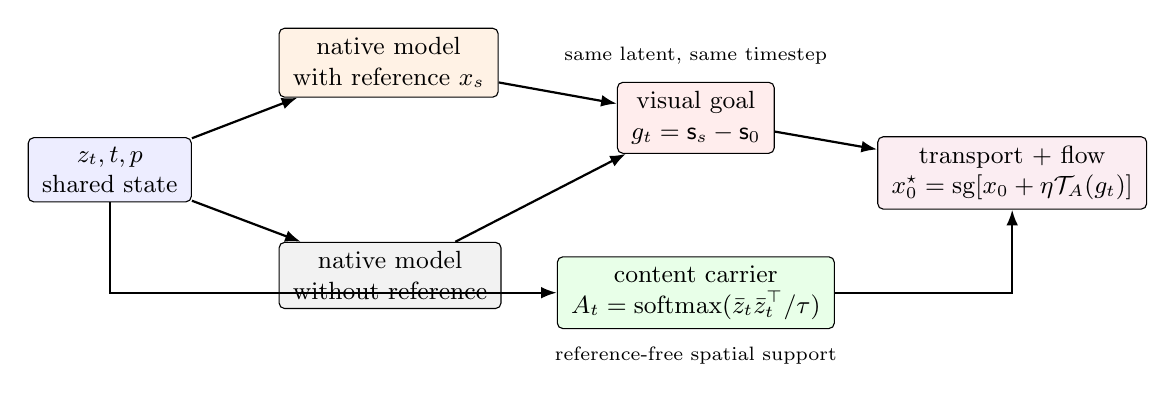
\begin{tikzpicture}[
  font=\small,
  box/.style={draw, rounded corners=2pt, minimum height=8mm, align=center,
              inner xsep=5pt, fill=white},
  arr/.style={-{Latex[length=2mm]}, thick},
  note/.style={font=\scriptsize, align=center}
]
\node[box, fill=blue!7] (state) {$z_t,t,p$\\shared state};
\node[box, fill=orange!10, above right=5mm and 11mm of state] (with)
  {native model\\with reference $x_s$};
\node[box, fill=gray!10, below right=5mm and 11mm of state] (without)
  {native model\\without reference};
\node[box, fill=red!7, right=15mm of with, yshift=-7mm] (goal)
  {visual goal\\$g_t=\score_s-\score_0$};
\node[box, fill=green!9, below=13mm of goal] (carrier)
  {content carrier\\$A_t=\mathrm{softmax}(\bar z_t\bar z_t^\top/\tau)$};
\node[box, fill=purple!7, right=13mm of goal, yshift=-7mm] (target)
  {transport + flow\\$x_0^\star=\sg[x_0+\eta\mathcal T_A(g_t)]$};
\draw[arr] (state) -- (with);
\draw[arr] (state) -- (without);
\draw[arr] (with) -- (goal);
\draw[arr] (without) -- (goal);
\draw[arr] (state.south) |- (carrier.west);
\draw[arr] (goal) -- (target);
\draw[arr] (carrier) -| (target);
\node[note, below=1mm of carrier] {reference-free spatial support};
\node[note, above=1mm of goal] {same latent, same timestep};
\end{tikzpicture}
}
\end{minipage}\hfill
\begin{minipage}[c]{0.42\textwidth}
\centering
\setlength{\tabcolsep}{2pt}
\begin{tabular}{ccc}
\includegraphics[width=0.31\linewidth]{formal25_score_carrier_start1000_score_carrier_style27_kp0_seed64_reference.png} &
\includegraphics[width=0.31\linewidth]{formal25_multi_kv_s27_kp0_seed64_kv_match_style27_kp0_seed64.png} &
\includegraphics[width=0.31\linewidth]{formal25_multi_score_carrier_s27_kp0_seed64_score_carrier_style27_kp0_seed64.png}\\[-1mm]
{\scriptsize Reference} & {\scriptsize K/V replacement} & {\scriptsize \method}\
\end{tabular}
\end{minipage}
\caption{\textbf{Goal, carrier, and flow.} Left: the reference changes only
the native goal branch; the spatial carrier is computed from the current
content state. Both teacher evaluations share the exact latent and timestep.
Right: for ``a panda eating bamboo,'' K/V replacement transfers appearance but
also inherits reference-like composition; \method{} retains the requested
content while expressing the reference palette and mark-making.}
\label{fig:overview}
\end{figure*}

\section{Related Work}

\paragraph{Style transfer and image conditioning.}
Classical neural style transfer matches feature statistics or adaptive moments
\cite{gatys2016style,huang2017adain}. Diffusion methods broaden the generative
prior through inversion, attention control, or exemplar conditioning
\cite{hertz2023prompt,tumanyan2023plugplay,yang2023paint}. Learned approaches
include low-rank style tuning and decoupled image-prompt adapters
\cite{sohn2023styledrop,ye2023ipadapter}. Training-free methods share or replace
attention features \cite{chung2024styleinjection,hertz2024stylealigned} or
inject image features into selected blocks \cite{wang2024instantstyle}. These
methods motivate our concern: appearance transfer is strongest when reference
features are spatially influential, precisely where reference-layout leakage
can arise. We use the model-native image condition to define appearance and a
separate content-state operator to define placement.

\paragraph{Guidance and score differences.}
Classifier guidance and classifier-free guidance alter a diffusion score by a
conditional contrast \cite{dhariwal2021diffusion,ho2022cfg}. Score Distillation
Sampling turns a frozen diffusion prior into an optimization gradient
\cite{poole2023dreamfusion}; Delta Denoising Score removes a matched source
direction for stable text-driven editing \cite{hertz2023dds}, and contrastive
variants add structure-preserving features \cite{nam2024cds}. Our residual is
related algebraically but differs in conditioning and use: both branches are
native image-edit evaluations at the current generated state, and their
reference-dependent difference is explicitly transported by a content-only
carrier before execution.

\paragraph{Distribution and flow matching.}
Diffusion and score models learn noise-conditional vector fields
\cite{ho2020ddpm,song2021sde}. Flow matching and rectified flow provide a direct
velocity parameterization \cite{lipman2023flow,liu2023rectified}, used by modern
multimodal diffusion transformers \cite{esser2024sd3}. Distribution Matching
Distillation (DMD) learns a fast generator from real and fake score differences
\cite{yin2024dmd,yin2024dmd2}. \method{} instead performs per-sample online
refinement and trains no generator. A dynamic fake-score term is compatible
with our carrier, but is not required by or claimed as the main method.

\section{Carrier-Anchored Image CFG}

\subsection{Problem and Same-State Contract}

Let $z_t\in\R^{L\times C}$ be the current noisy image tokens, $t$ the sampler
timestep, $p$ a content prompt, and $x_s$ a style reference. The frozen native
edit model predicts velocity $\vel_s(z_t,t,p,x_s)$ when shown the reference and
$\vel_0(z_t,t,p)$ when the reference condition is removed. The two evaluations
must share the same $z_t$, $t$, prompt metadata, and image-token IDs. Otherwise,
their difference contains an uncontrolled state change and cannot be
interpreted as guidance.

For the flow scheduler
\begin{equation}
 z_\sigma=(1-\sigma)x_0+\sigma\epsilon,\qquad
 \vel=\epsilon-x_0,
 \label{eq:flow}
\end{equation}
we have $\hat x_0=z_\sigma-\sigma\vel$ and
$\score=-(z_\sigma+(1-\sigma)\vel)/\sigma$. Shared state terms cancel, giving
\begin{equation}
 g_t \equiv \score_s-\score_0
 =-\frac{1-\sigma}{\sigma}(\vel_s-\vel_0).
 \label{eq:goal}
\end{equation}
The implementation resolves $\sigma$ from the scheduler table, clamps only its
degenerate endpoint, and sets the correction to zero when the inverse
conversion is undefined.

Equation~\ref{eq:goal} is an image analogue of CFG. If the two branches
estimate conditional densities $p_s$ and $p_0$, then
\begin{equation}
 g_t=\nabla_{z_t}\log p_s(z_t\mid p,x_s)
     -\nabla_{z_t}\log p_0(z_t\mid p)
 =\nabla_{z_t}\log\frac{p_s}{p_0}.
 \label{eq:ratio}
\end{equation}
Thus the native model, rather than replaced K/V tensors or a learned adapter,
defines what the reference asks the current sample to change.

\subsection{Reference-Independent Spatial Carrier}

A goal is not yet a rendering rule. We compute a token affinity from the saved
post-scheduler content state $c_t$:
\begin{equation}
 A_t=\operatorname{softmax}\!\left(\frac{\bar c_t\bar c_t^\top}{\tau}\right),
 \qquad \bar c_{t,u}=\frac{c_{t,u}}{\lVert c_{t,u}\rVert_2}.
 \label{eq:affinity}
\end{equation}
$A_t$ is detached and never receives $x_s$. It is therefore a spatial carrier,
not another style extractor. The transported field is
\begin{equation}
 \mathcal T_A(g_t)=g_t+\lambda_A(A_tg_t-g_t),
 \label{eq:transport}
\end{equation}
with an optional high-pass residual in the general implementation. The formal
configuration uses no high-pass gain, isolating affinity transport.

This design gives CA a specific role. The model's native image-conditioning
path, which includes its cross-attention machinery, forms $g_t$. The explicit
content affinity then decides which current-image tokens share that change.
Reference K/V tensors are not inserted into $A_t$; consequently the carrier
cannot directly reproduce the reference arrangement.

\subsection{Online Objective}

We optimize the current latent, not model parameters. The base branch predicts
$\hat x_0^0=z_t-\sigma\vel_0(z_t)$ with gradients retained through
$\vel_0$. The styled branch is detached. The direct goal-matching term is
\begin{equation}
 \mathcal L_{\mathrm{goal}}
 =\left\lVert\mathcal N\!\left[
 -\frac{1-\sigma}{\sigma}
 \big(\vel_0(z_t)-\sg[\vel_s(z_t)]\big)
 \right]\right\rVert_2^2,
 \label{eq:lgoal}
\end{equation}
where $\mathcal N$ removes the timestep scalar magnitude while preserving field
direction and relative token energy.

For the carrier term, we form a detached pseudo-target
\begin{equation}
 x_0^\star=\sg\left[\hat x_0^0+
 \eta\,\operatorname{RMSNorm}(\mathcal T_A(g_t))\right],
 \quad
 \mathcal L_{\mathrm{carrier}}=\tfrac12
 \lVert\hat x_0^0-x_0^\star\rVert_2^2.
 \label{eq:carrierloss}
\end{equation}
The complete per-sample objective is
\begin{equation}
 \mathcal L=\mathcal L_{\mathrm{goal}}
 +\lambda_c\mathcal L_{\mathrm{carrier}}
 +\lambda_d\mathcal L_{\mathrm{dist}}
 +\lambda_p\mathcal L_{\mathrm{content}}.
 \label{eq:full}
\end{equation}
The last two terms are inherited safeguards that keep the local score direction
within the valid sample neighborhood. All teacher fields, affinities, and
pseudo-directions are detached at their stated boundaries. AdamW updates only
$z_t$; with zero weight decay it is numerically Adam, while exposing decay as a
separate regularization ablation.

\begin{figure}[t]
\centering
\fbox{\begin{minipage}{0.94\columnwidth}
\small
\textbf{One \method{} step at $(z_t,t)$.}

1. Save the post-scheduler state and resolve its exact $\sigma$.

2. Evaluate $\vel_s$ and $\vel_0$ on that same state; form $g_t$ using
Eq.~\ref{eq:goal}.

3. Build detached $A_t$ from content tokens only and transport $g_t$ by
Eq.~\ref{eq:transport}.

4. Construct $x_0^\star$, update $z_t$ with Eq.~\ref{eq:full}, then advance
the original flow sampler.
\end{minipage}}
\caption{The online algorithm. The reference is encoded once; no network
parameters or persistent adapter state are optimized.}
\label{fig:algorithm}
\end{figure}

\subsection{Why Not K/V Replacement or an Adapter?}

K/V replacement defines both appearance and token correspondence with the
reference. Its visual effect can be strong, but a failure cannot be attributed
cleanly to the goal or the carrier. \method{} instead obtains a whole-model
reference contrast and then imposes content-state correspondence. An adapter
could amortize this computation for repeated serving, but it would answer a
different question: whether a trainable network can predict the field. The
main method asks whether the native field can be exposed and used online for a
single reference. No special training set is necessary.

\section{Experiments}

\subsection{Protocol}

We evaluate on Klein9B at $512\times512$. The controlled set contains three
style references paired with three content prompts (castle, sunflower field,
and panda), using a fixed seed for the matched teacher comparison. The
representative audit uses style 27, ``a panda eating bamboo,'' and seed 64.
Every compared branch uses 25 outer flow steps, a dynamic 5-to-2 inner schedule,
start time 1000, AdamW with zero latent decay, and no warm-start style-transport
or AdaIN color-matching heuristics. The
formal \method{} setting uses distance weight 0.3, content weight 0.4, carrier
temperature 0.1, strength 0.75, high-pass gain 0, and carrier-loss weight 0.25.

We report CSD style similarity \cite{somepalli2024csd}, CLIP text alignment
\cite{radford2021clip}, DINO style similarity \cite{oquab2024dinov2}, VGG Gram
distance, and DINO self-similarity correlation with the reference (layout
leakage). The first three are higher-is-better; Gram and leakage are
lower-is-better. Because raw CSD is not a calibrated universal style metric
\cite{frochte2026csd}, conclusions require agreement with qualitative results
and the other metrics. All evaluator checkpoints and preprocessing hashes are
recorded.

\paragraph{Baselines.}
\emph{K/V replacement} is the standard training-free attention-feature
replacement baseline \cite{hertz2024stylealigned,chung2024styleinjection}, which
substitutes reference key and value tensors into self-attention.
\emph{Score match} optimizes Eq.~\ref{eq:lgoal} without explicit transport.
\emph{Score carrier} is \method. The strict audit reruns the final configuration
from an isolated trial copy. CA+DMD is excluded from the headline comparison:
it requires a persistent, dynamically updated fake-score model and is not
equivalent to simply adding a frozen score term.

\subsection{Does the Native Goal Improve over K/V Replacement?}

Table~\ref{tab:formal} reports the representative pair. Native score matching
raises CSD from 0.5614 to 0.6770. Adding the carrier reaches 0.6882 and improves
Gram distance and layout leakage relative to score-only matching. A fresh
strict run obtains 0.6896 CSD, confirming that the result is not a stale metric
artifact.

\begin{table}[t]
\centering
\caption{Representative matched comparison. Bold marks the best non-audit
method; the audit independently reruns \method.}
\label{tab:formal}
\small
\setlength{\tabcolsep}{3.2pt}
\begin{tabular}{lrrrrr}
\toprule
Method & CSD$\uparrow$ & CLIP$\uparrow$ & DINO$\uparrow$ & Gram$\downarrow$ & Leak$\downarrow$\\
\midrule
K/V replace & .5614 & .3465 & .0677 & 2.9437 & .2893\\
Score match & .6770 & \textbf{.3476} & \textbf{.0749} & 2.4451 & .3018\\
\method & \textbf{.6882} & .3282 & .0727 & \textbf{2.2915} & \textbf{.2780}\\
Strict audit & .6896 & .3375 & .0740 & 2.3901 & .2805\\
\bottomrule
\end{tabular}
\end{table}

\begin{figure*}[t]
\centering
\setlength{\tabcolsep}{3pt}
\begin{tabular}{ccc}
\includegraphics[width=0.205\textwidth]{formal25_multi_score_carrier_s00_kp1_seed64_score_carrier_style00_kp1_seed64_reference.png} &
\includegraphics[width=0.205\textwidth]{formal25_multi_kv_s00_kp1_seed64_kv_match_style00_kp1_seed64.png} &
\includegraphics[width=0.205\textwidth]{formal25_multi_score_carrier_s00_kp1_seed64_score_carrier_style00_kp1_seed64.png}\\[-1mm]
{\scriptsize Reference 00} & {\scriptsize K/V: castle, CSD .470} & {\scriptsize \method: castle, CSD .673}\\[1mm]
\includegraphics[width=0.205\textwidth]{formal25_multi_score_carrier_s13_kp3_seed64_score_carrier_style13_kp3_seed64_reference.png} &
\includegraphics[width=0.205\textwidth]{formal25_multi_kv_s13_kp3_seed64_kv_match_style13_kp3_seed64.png} &
\includegraphics[width=0.205\textwidth]{formal25_multi_score_carrier_s13_kp3_seed64_score_carrier_style13_kp3_seed64.png}\\[-1mm]
{\scriptsize Reference 13} & {\scriptsize K/V: sunflowers, CSD .313} & {\scriptsize \method: sunflowers, CSD .335}\\[1mm]
\includegraphics[width=0.205\textwidth]{formal25_multi_score_carrier_s27_kp0_seed64_score_carrier_style27_kp0_seed64_reference.png} &
\includegraphics[width=0.205\textwidth]{formal25_multi_kv_s27_kp0_seed64_kv_match_style27_kp0_seed64.png} &
\includegraphics[width=0.205\textwidth]{formal25_multi_score_carrier_s27_kp0_seed64_score_carrier_style27_kp0_seed64.png}\\[-1mm]
{\scriptsize Reference 27} & {\scriptsize K/V: panda, CSD .426} & {\scriptsize \method: panda, CSD .691}
\end{tabular}
\caption{Matched qualitative comparison for all three reported pairs. Columns
are reference, K/V replacement, and \method; prompt and seed are fixed within
each row. The method's largest gains occur for references 00 and 27, while
reference 13 exposes a difficult, nearly neutral case. This heterogeneity is
why we report per-pair values and do not infer broad dominance from the mean.}
\label{fig:qualitative}
\end{figure*}

\paragraph{Per-reference behavior.}
Figure~\ref{fig:qualitative} exposes variation hidden by the average. The CSD
gains over K/V replacement are $+0.2031$, $+0.0222$, and $+0.2650$ for styles
00, 13, and 27. Text alignment changes by $+0.0047$, $-0.0052$, and $+0.0035$,
respectively. The near-tie on style 13 is scientifically useful: a native goal
does not guarantee that the chosen content carrier is appropriate for every
reference. A larger study should stratify references by spatial frequency,
palette concentration, and semantic content rather than report only a pooled
mean.

The result separates two improvements. The native image-CFG residual provides
the large style gain over attention replacement. Carrier anchoring then changes
where that signal acts, recovering the lowest leakage in this matched record.
The CLIP-T decrease shows that carrier strength is a trade-off rather than a
free scalar improvement.

\subsection{Matched Multi-Reference Result}

Table~\ref{tab:threepair} holds reference, prompt, seed, sampler, and loss
weights fixed across three pairs. \method{} improves mean CSD by 0.1635 and DINO
style similarity by 0.0143 over K/V replacement, while CLIP-T remains
effectively unchanged. Gram distance and layout leakage are slightly worse,
revealing that stronger native style transfer is not identical to stricter
content conservation. We therefore claim a stronger style signal, not universal
Pareto dominance.

\begin{table}[t]
\centering
\caption{Three-pair matched means (one seed per pair). Standard deviations are
shown for CSD; a full matched multi-seed matrix remains a submission gate.}
\label{tab:threepair}
\small
\setlength{\tabcolsep}{3.4pt}
\begin{tabular}{lrrrrr}
\toprule
Method & CSD$\uparrow$ & CLIP$\uparrow$ & DINO$\uparrow$ & Gram$\downarrow$ & Leak$\downarrow$\\
\midrule
K/V replace & .4027$\pm$.0660 & .3286 & .0476 & \textbf{4.0299} & \textbf{.3352}\\
\method & \textbf{.5662$\pm$.1635} & \textbf{.3296} & \textbf{.0619} & 4.0891 & .3479\\
\bottomrule
\end{tabular}
\end{table}

\subsection{What Makes the Carrier Work?}

\paragraph{Start time.}
At start time 850, score matching obtains 0.4278 CSD; at 1000, the same
objective obtains 0.6770. The carrier cannot recover a goal that is weak or
introduced after too much content has already crystallized. The result supports
early access to the native style residual, but does not by itself establish a
particular transformer layer at which style ``appears.'' Layerwise emergence is
therefore a future causal-probe question, not a premise of the method.

\paragraph{Carrier versus score-only.}
On the representative case, carrier anchoring changes CSD from 0.6770 to
0.6882, Gram from 2.4451 to 2.2915, and leakage from 0.3018 to 0.2780. This is
the causal comparison for the carrier: both rows use the same native goal and
differ by the content-affinity pseudo-target. The gain is modest relative to
the goal extraction itself, but it is consistent across the three metrics that
measure style statistics and spatial copying on this case.

\paragraph{Optimizer regularization.}
A single-pair sweep gives CSD 0.6764 for Adam, 0.6758 for AdamW with zero decay,
0.7045 for decay $10^{-4}$, and 0.6813 for $10^{-3}$. However, over three pairs,
$10^{-4}$ changes mean CSD from 0.5662 to 0.5607. We therefore use zero decay
and report nonzero decay only as an explicit latent regularizer. This avoids
selecting a headline setting from one favorable reference.

\subsection{Mechanism Audit}

The decomposition yields interventions that a monolithic feature-injection
method does not. Table~\ref{tab:claims} separates established observations from
open claims. In particular, the start-time result concerns noise level, not
network depth. We deliberately do not claim that a specific transformer layer
first represents style until layer probes and causal activation swaps are run.

\begin{table}[t]
\centering
\caption{Claim--evidence audit. ``Limited'' means the intervention is valid but
the sample coverage is not yet sufficient for a broad claim.}
\label{tab:claims}
\small
\setlength{\tabcolsep}{3pt}
\begin{tabular}{p{0.22\columnwidth}p{0.43\columnwidth}p{0.23\columnwidth}}
\toprule
Claim & Controlled evidence & Status\\
\midrule
Native goal is useful & Same-state score vs. K/V; $+0.1635$ mean CSD & Supported on 3 pairs\\
Carrier changes placement & Score-only vs. carrier; leak $.3018\!\to\!.2780$ & Limited to formal pair\\
Goal benefits from early noise & Start $850\!\to\!1000$; CSD $.4278\!\to\!.6770$ & Limited to formal pair\\
Carrier excludes reference layout & Reference tensor absent from Eq.~\ref{eq:affinity} and asserted in code & By construction\\
Broad generalization & Matched multi-seed and human study & Not yet established\\
\bottomrule
\end{tabular}
\end{table}

\paragraph{Detach-boundary check.}
The teacher branch is not differentiated through, and the shared
$-z_t/\sigma$ score term is removed analytically before detachment. This avoids
an identity gradient that would appear if two full scores were independently
formed and subtracted after one branch had been detached. Gradients enter
through $\vel_0(z_t)$ in Eq.~\ref{eq:lgoal} and through $\hat x_0^0(z_t)$ in
Eq.~\ref{eq:carrierloss}; the native residual and affinity remain target data.
This implementation detail is central to reproducing the intended score
matching objective.

\paragraph{Carrier limiting cases.}
When $\lambda_A=0$, Eq.~\ref{eq:transport} reduces to score-only guidance. When
$A_t=I$, increasing carrier strength has no effect. A uniform $A_t$ collapses
token-specific directions toward a global style field, while a reference-based
$A_t$ reintroduces the layout-copying path we seek to remove. These cases give
simple unit tests for identity, smoothing, and reference-independence.

\subsection{Online Refinement, DMD, and Amortization}

The word ``distillation'' can refer to three different optimization objects.
Table~\ref{tab:modes} makes the distinction explicit. \method{} distills a frozen
native score contrast into the current sample in real time. It does not train a
global adapter. A field student is optional amortization. A CA+DMD extension
additionally estimates a fake-distribution score and therefore has a different
state and update contract.

\begin{table}[t]
\centering
\caption{Optimization contracts. Only the first row is the main method.}
\label{tab:modes}
\small
\setlength{\tabcolsep}{3pt}
\begin{tabular}{llll}
\toprule
Mode & Optimized & Persistent & Data\\
\midrule
\method & current $z_t$ & none & one sample/reference\\
Field student & $G_\theta$ & student weights & dumped teacher fields\\
CA+DMD & $z_t$, fake score & critic state & online fake samples\\
\bottomrule
\end{tabular}
\end{table}

For CA+DMD, a valid additional direction has the form
\begin{equation}
 g_t^{\mathrm{total}}=\lambda_A\mathcal T_A(g_t)
 +\lambda_{\mathrm{DM}}\big(\score_s-\score_{\mathrm{fake},\phi}\big).
 \label{eq:dmdext}
\end{equation}
The fake scorer $\phi$ must persist and be refreshed on current generated
states; resetting it or replacing it with a fixed model is not DMD. Our code
exposes this extension and rejects CA+DMD when no real fake-score backend is
configured. Since current controlled results do not establish a gain, it is an
extension rather than part of the headline claim.

An optional student $G_\theta(z_t,t,p,E(x_s))$ can regress the transported
field for repeated use. A deterministic VAE image code reaches field cosine
0.4988 versus 0.4486 for a style-ID code in the random matched split, but the
held-out-style comparison is nearly tied (0.3094 vs. 0.3164). This confirms a
real-image interface without establishing universal out-of-style
generalization; full details belong in the supplement.

\subsection{Properties of the Carrier}

The simple affinity in Eq.~\ref{eq:affinity} has two useful properties. They do
not prove image-quality improvement, but they state exactly what the carrier
can and cannot introduce.

\paragraph{Reference independence.}
Let $A_t=F(c_t)$ for deterministic $F$, and hold the current content state
$c_t$ fixed while changing the reference. Then
$\partial A_t/\partial x_s=0$. Consequently, the reference can change
$\mathcal T_A(g_t)$ only through the goal $g_t$; it cannot change the transport
operator itself. This is weaker than saying the final image cannot resemble the
reference, since resemblance may be encoded in the native goal. It is stronger
than K/V replacement in one precise respect: there is no direct path from
reference token geometry to the explicit carrier.

\paragraph{Non-expansion of token energy.}
Each row of $A_t$ is nonnegative and sums to one. For
$0\leq\lambda_A\leq1$, Eq.~\ref{eq:transport} is also a convex token-mixing
operator. With $\lVert g\rVert_{\infty,2}=\max_u\lVert g_u\rVert_2$,
\begin{equation}
 \lVert\mathcal T_A(g)\rVert_{\infty,2}
 \leq \lVert g\rVert_{\infty,2}.
 \label{eq:stability}
\end{equation}
Indeed, each output token is a convex combination of input goal tokens, so the
triangle inequality gives Eq.~\ref{eq:stability}. The carrier can redistribute
a strong native residual, but before the explicit RMS normalization it cannot
create a larger token vector than the field already contains. This helps
separate spatial transport from guidance-scale amplification.

These properties explain why we keep carrier strength in $[0,1]$ in the formal
protocol. High-pass gains or extrapolative strengths above one may improve
texture, but they forfeit the stability statement and must be evaluated as
separate appearance amplifiers.

\subsection{Training Cost, Reproducibility, and Boundaries}

The method has no parameter-training stage. Each online inner iteration adds
native with-reference and without-reference evaluations plus latent
backpropagation; cost scales with flow steps and inner iterations. An optional
image-code student can amortize the field for repeated deployment, but is
reported only in the supplement and is not part of \method.

Every result is keyed by reference path, prompt, seed, saved latent, timestep,
scheduler sigma, model roots, loss weights, optimizer configuration, and
evaluator hashes. Positive and negative native branches are asserted to share
the post-scheduler state. Generated artifacts, manifests, and the isolated
reward trial live inside the project repository. An external read-only source
tree is never modified.

Two boundaries matter. First, the present matched comparison is small; a
multi-seed, larger-reference benchmark and human preference study are required
before claiming broad superiority. Second, a frozen image metric on a noisy
intermediate decode is not a value function. In our supplementary diagnostic,
greedy CSD-based action selection does not beat the 0.6896 baseline, even under
a same-state local oracle. This does not contradict final-image best-of-$N$;
the candidates were not rolled out to final images before selection.

\subsection{Failure Modes and Evaluation Scope}

\paragraph{Goal and carrier failures.}
The carrier cannot invent a style direction absent from the native contrast,
and a reference with a dominant object may place semantics inside $g_t$ along
with appearance. Meanwhile, cosine transport can smooth high-frequency changes
across visually similar tokens that belong to different objects. The difficult
style-13 row in Figure~\ref{fig:qualitative} is consistent with these limits.
Sparse, object-aware, or multiscale carriers are plausible extensions if their
transport operator remains reference-independent.

\paragraph{Evaluation and use.}
CSD, CLIP-T, Gram statistics, and DINO self-similarity each capture only part of
style fidelity and content preservation. The three-pair study is therefore a
mechanism test, not a definitive benchmark; matched multi-seed evaluation and
blinded human comparison remain necessary. Online refinement also trades
training cost for repeated inference-time model evaluations. Finally,
reference-conditioned style systems can facilitate imitation of living
artists. Dataset licenses, opt-out policies, and attribution analysis should
accompany deployment; CSD is not evidence of authorship or ownership.

\section{Discussion and Conclusion}

\method{} turns a reference image into an explicit, testable operation. The
native score contrast says what visual change the reference requests; a
reference-independent affinity says where that change can be rendered in the
current scene; the flow parameterization says how it becomes a denoising
update. This resolves the role of CA without introducing an adapter: native
cross attention participates in goal formation, while the explicit carrier
anchors spatial execution.

The current evidence supports the mechanism on controlled cases and exposes
its trade-offs rather than hiding them. The next decisive experiment is not a
more elaborate loss, but a larger matched matrix that tests whether carrier
anchoring consistently improves the style--layout frontier. More expressive
content-only transport and final-trajectory reward selection are natural
extensions. The central principle remains simple: thinking with a reference
image requires separating the visual goal from the spatial carrier that makes
it executable.

\clearpage
\bibliographystyle{plain}
\bibliography{AAAI/references}

\clearpage
\section{Reproducibility Checklist}
\small

This paper follows the AAAI reproducibility checklist. Unless noted, section and
figure references point to the main paper; ``released code'' refers to the
anonymized code and manifests accompanying this submission.

\paragraph{General.}
\begin{itemize}\itemsep1pt
\item Conceptual outline / pseudocode of the AI methods introduced: \textbf{yes}
(Method \S3; pseudocode in the Algorithm subsection of this appendix).
\item Delineates opinions / hypotheses / speculation from objective facts:
\textbf{yes} (the regularization substitution is stated as an empirical finding,
not a theorem; boundaries stated in Limitations).
\item Well-marked pedagogical references for less-familiar readers: \textbf{yes}
(rectified flow, classifier-free guidance, distribution-matching distillation,
and classical style transfer are cited).
\end{itemize}

\paragraph{Theoretical contributions.} The paper makes no formal theoretical
contribution (\textbf{no}). Its claims are empirical by design; the
velocity-contrast$=$score-difference relation used in \S3 is a derivation from
standard tools with citations, and the reverse-process regularization is
explicitly an empirical finding (\S Conclusion), not a theorem. Accordingly the
theorem/proof items are not applicable; the corresponding empirical evidence
(reverse-step ablation, fake-score negative study, rejected SRSD metric) and its
code are included.

\paragraph{Datasets.} The paper relies on a fixed style-reference set (\textbf{yes}).
\begin{itemize}\itemsep1pt
\item Motivation for the selected data: \textbf{yes} (a media-diverse
40-reference library isolates medium transfer across style locality).
\item Novel data included in a data appendix: \textbf{partial} (style IDs,
prompts, seeds, candidate order, and evaluator inputs are retained in
machine-readable manifests in the released code; reference images are model-
generated and described).
\item Novel data public on publication with a license: \textbf{partial}
(intended; redistribution and license terms to be finalized before release).
\item Existing-literature datasets cited / public: \textbf{NA} (no external
benchmark dataset is used; the reference set and content prompt are constructed
here).
\item Non-public data described in detail: \textbf{yes} (all style IDs, the
content prompt, seeds, and evaluator inputs are specified).
\end{itemize}

\paragraph{Computational experiments.} The paper includes computational
experiments (\textbf{yes}).
\begin{itemize}\itemsep1pt
\item Number and range of (hyper-)parameter values tried during development:
\textbf{yes} (the parameter study sweeps step count, inner iterations, step
size, and normalization; grids in this appendix).
\item Pre-processing code included: \textbf{partial} (generation and evaluation
code is in the released code; pre-processing is minimal).
\item All source code for running and analyzing experiments included:
\textbf{partial} (released with the submission; generation, matched native
baseline, sweeps, the reverse-step ablation, Agent evaluation, aggregation, and
figure/table builds are covered).
\item Source code public on publication with a license: \textbf{yes} (intended).
\item New-method code has comments referencing the paper: \textbf{partial}.
\item Method for setting seeds described: \textbf{yes} (a single fixed seed, 65,
is used throughout and stated).
\item Computing infrastructure specified: \textbf{partial} (single-GPU
inference, bf16, AdamW with zero latent weight decay; exact library versions are
pinned in the released environment).
\item Evaluation metrics formally described with motivation: \textbf{yes} (CSD,
CLIP-T, and layout-leak are defined and motivated as separable style / subject /
composition axes; \S4).
\item Number of algorithm runs per reported result stated: \textbf{yes}
(fixed-seed; one run per task$\times$style cell over $n=40$ references).
\item Analysis beyond single-number summaries: \textbf{yes} (per-style values,
cross-style SD, 95\% style-bootstrap intervals, 40/40 paired-win counts, and the
CSD--CLIP-T frontier).
\item Significance judged with appropriate statistical tests: \textbf{partial}
(style-bootstrap confidence intervals, paired-win counts, and cross-Agent
correlation statistics; we do not run a formal null-hypothesis test on the main
metric and we do not claim random-seed uncertainty).
\item All final (hyper-)parameters listed: \textbf{yes} (per-mode step count,
inner iterations, step size, and normalization are tabulated in this appendix).
\end{itemize}
\normalsize


\end{document}
